\documentclass{pginz}
%%%%%%%%%Miejsce na dodatkowe pakiety%%%%%%%%%%%%%
\usepackage{subcaption}
\PassOptionsToPackage{polish}{babel}
\usepackage{babel}
\usepackage[utf8]{inputenc}  % For UTF-8 support
\usepackage{makecell}
\usepackage{tikz}
\usepackage{circuitikz}
\usepackage{algorithm}
\usepackage{algpseudocode}
\usepackage{pgfplots}
\pgfplotsset{compat=1.18}
\usepackage[T1]{fontenc}
\usepackage{lmodern}
\usepackage{mathpazo}
\usepackage{textcomp}
\DeclareTextSymbol{\textOslash}{T1}{216}
\newcommand{\Oslash}{\textOslash}
\usepackage{url}
\urlstyle{same}

\pdfstringdefDisableCommands{\let\HyPsd@CatcodeWarning\@gobble}

\begin{document}

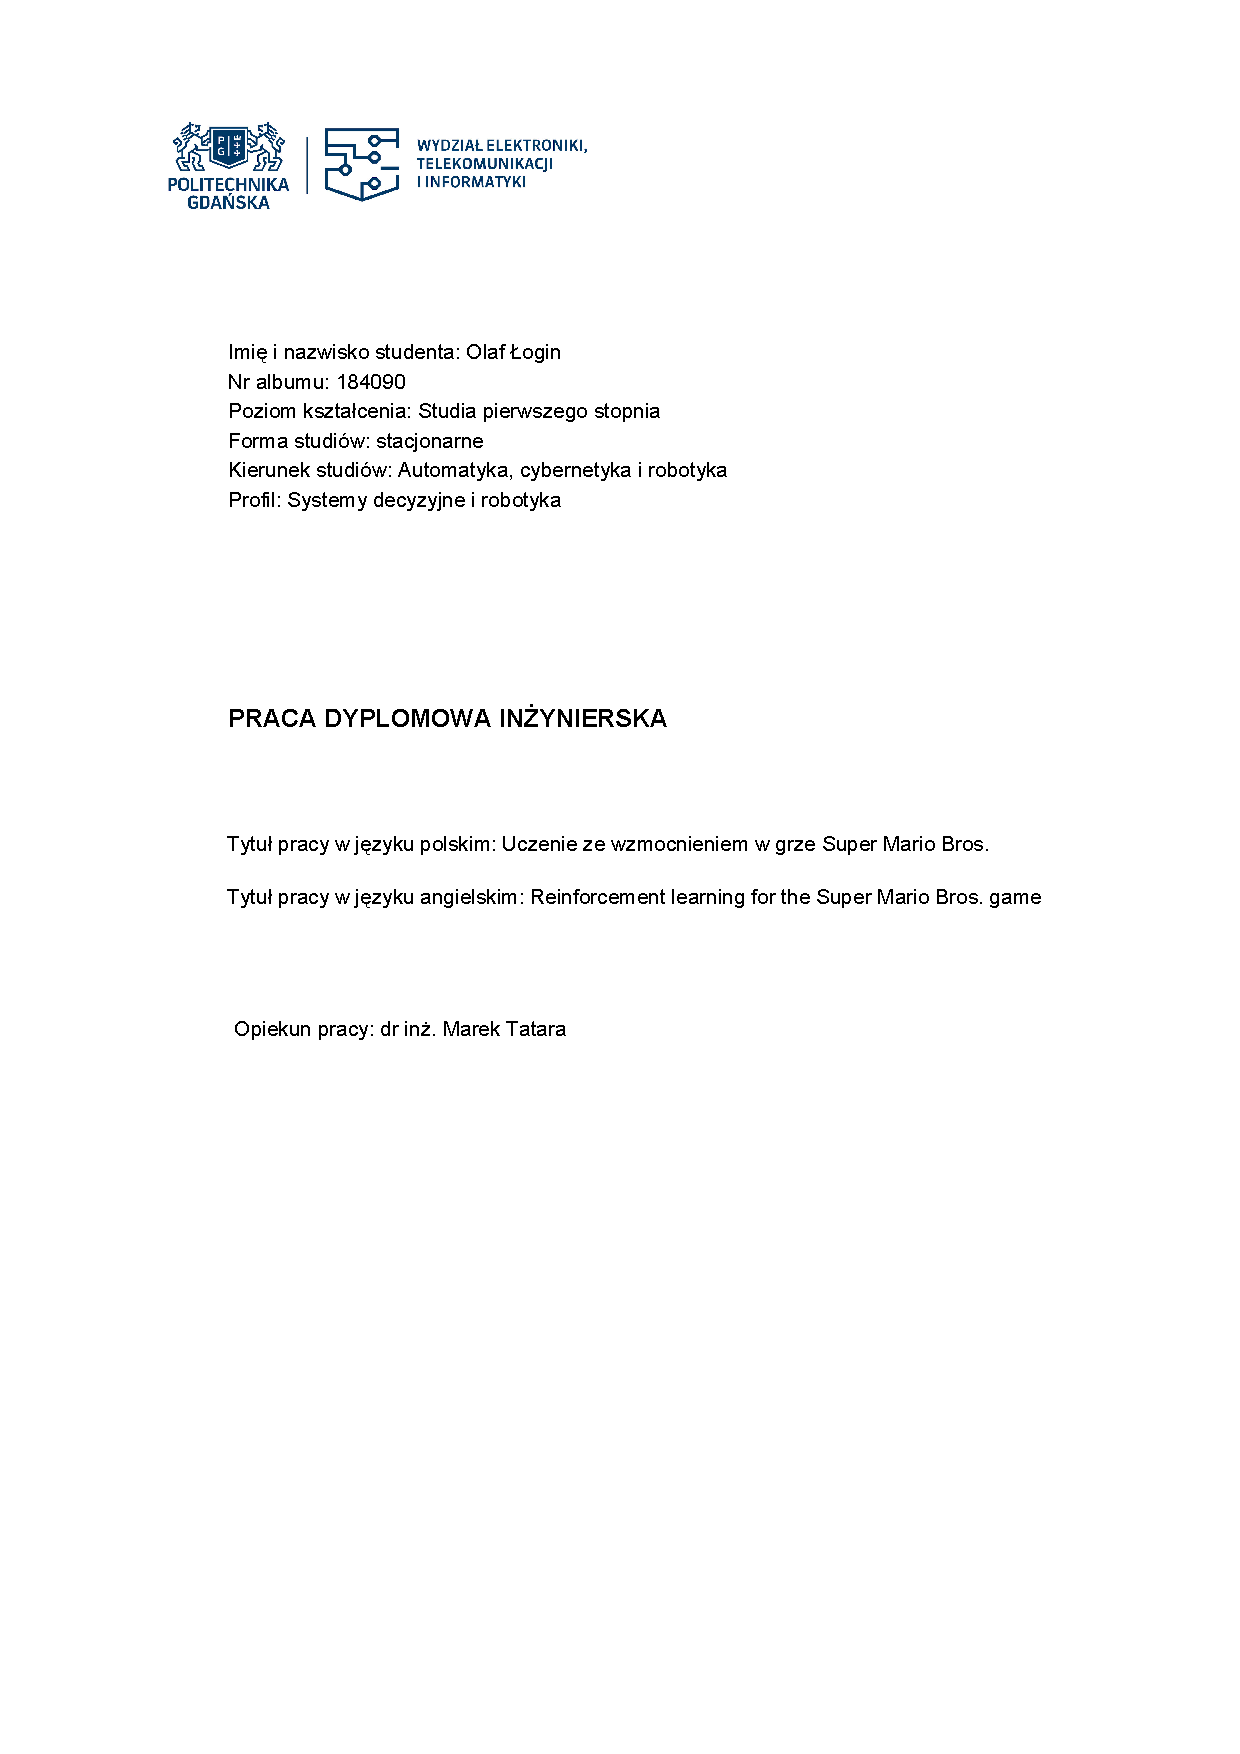
\includepdf{assets/StronaTytulowa.pdf}
%\includepdf[page={1}]{Oswiadczenie.pdf}

\setcounter{page}{2}

\chapter*{Streszczenie}

Lorem ipsum dolor sit amet, consectetuer adipiscing elit, sed diam nonummy nibh euismod tincidunt ut laoreet dolore magna aliquam erat volutpat. Ut wisi enim ad minim veniam, quis nostrud exerci tation ullamcorper suscipit lobortis nisl ut aliquip ex ea commodo consequat. Duis autem vel eum iriure dolor in hendrerit in vulputate velit esse molestie consequat, vel illum dolore eu feugiat nulla facilisis at vero eros et accumsan et iusto odio dignissim qui blandit praesent luptatum zzril delenit augue duis dolore te feugait nulla facilisi. Nam liber tempor cum soluta nobis eleifend option congue nihil imperdiet doming id quod mazim placerat facer possim assum. Typi non habent claritatem insitam; est usus legentis in iis qui facit eorum claritatem. Investigationes demonstraverunt lectores legere me lius quod ii legunt saepius. Claritas est etiam processus dynamicus, qui sequitur mutationem consuetudium lectorum. Mirum est notare quam littera gothica, quam nunc putamus parum claram, anteposuerit litterarum formas humanitatis per seacula quarta decima et quinta decima. Eodem modo typi, qui nunc nobis videntur parum clari, fiant sollemnes in futurum.

\bigskip

\noindent\textbf{Słowa kluczowe:} lorem ipsum, sterowanie cyfrowe, ...

\bigskip

\noindent\textbf{Dziedzina nauki i techniki zgodna z OECD} Nauki inżynieryjne i techniczne, Elektrotechnika, elektronika i inżynieria informatyczna, Robotyka i Automatyka

\chapter*{Abstract}

\noindent\textbf{Reinforcement learning for the Super Mario Bros. game}
The aim of this engineering thesis was to develop and evaluate a reinforcement learning-based model capable of completing levels in the \textit{Super Mario Bros} game. The implementation utilized the Double Q-Learning algorithm, a convolutional neural network, and the Weights and Biases tool for experiment monitoring. The thesis analyzed the impact of training parameters, such as the discount factor, epsilon decay strategy, and reward function, on model performance. The results confirm that appropriate parameter tuning and a balanced reward function significantly enhance the algorithm's efficiency.


\tableofcontents
\addcontentsline{toc}{chapter}{Spis treści}

\chapter*{Lista symboli}

\begin{itemize}[noitemsep,topsep=0pt,parsep=0pt,partopsep=0pt,labelwidth=1cm,align=left,itemindent=0pt]
	% Oznaczenia
	\item \(\epsilon\) - Współczynnik eksploracji w strategii \(\epsilon\)-greedy
	\item \(\epsilon_d\) - Tempo wygaszania współczynnika eksploracji (\(\epsilon\))
	\item \(\gamma\) - Współczynnik dyskontowy uwzględniający przyszłe nagrody
	\item \(Q(s, a)\) - Funkcja wartości akcji dla stanu \(s\) i akcji \(a\)
	\item \(x_{\text{pos}}\) - Pozycja Mario na osi poziomej
	\item \(r_t\) - Nagroda uzyskana w kroku \(t\)
	\item \(L(\theta)\) - Funkcja kosztu (loss) modelu z parametrami \(\theta\)
	\item \(y_t\) - Wartość docelowa w kroku \(t\)

\end{itemize}

\chapter*{Lista skrótów}

\begin{itemize}[noitemsep,topsep=0pt,parsep=0pt,partopsep=0pt,labelwidth=1cm,align=left,itemindent=0pt]
	% Skróty
	\item \textbf{DQN} - Deep Q-Network (Głęboka sieć Q)
	\item \textbf{RL} - Reinforcement Learning (Uczenie ze wzmocnieniem)
	\item \textbf{SQL} - SQLite (Lekka baza danych)
	\item \textbf{CNN} - Convolutional Neural Network (Konwolucyjna sieć neuronowa)
	\item \textbf{WandB} - Weights and Biases (Narzędzie do monitorowania i wizualizacji eksperymentów)
	\item \textbf{Replay Buffer} - Bufor odtworzeń przechowujący doświadczenia agenta
	\item \textbf{MSE} - Mean Squared Error (Błąd średniokwadratowy)
\end{itemize}


\chapter{Wstęp}

\section{Cel pracy}
Celem projektu inżynierskiego jest opracowanie programu opartego na uczeniu maszynowym, zdolnego do samodzielnego rozwiązywania problemów występujących w grze \textit{Super Mario Bros} na platformie Nintendo Entertainment System (NES).
Projekt obejmuje badanie zastosowania algorytmów uczenia ze wzmocnieniem oraz analizę efektywności różnych podejść w symulowanym środowisku gry.

\section{Opis gry \textit{Super Mario Bros}}

\textit{Super Mario Bros} to klasyczna gra platformowa wydana przez Nintendo w 1985 roku na konsolę NES.
Celem gry jest przejście bohaterem, Mario, z lewej strony ekranu na prawą, aż do końca poziomu, gdzie zwykle znajduje się flaga oznaczająca jego ukończenie.
Gracz musi pokonać serię poziomów.

Podczas gry Mario napotyka różnorodne przeszkody, wrogów oraz pułapki.
Do głównych zagrożeń należą przeciwnicy, tacy jak Goomba i Koopa Troopa, przepaście oraz spadające platformy.
Aby unikać zagrożeń lub je eliminować, Mario może skakać na wrogów lub korzystać z przedmiotów zwiększających jego zdolności, takich jak grzyby, które powiększają postać, czy kwiaty ognia umożliwiające atakowanie przeciwników z dystansu.

Kluczową mechaniką gry jest precyzyjne poruszanie się i planowanie kolejnych ruchów, ponieważ niewłaściwe decyzje często prowadzą do przegranej.

\begin{figure}[h!]
	\centering
	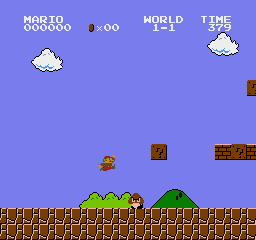
\includegraphics[width=0.8\textwidth]{img/screenshot_mario.png}
	\caption{Przykładowy ekran z gry \textit{Super Mario Bros.}}
	\label{fig:screenshot_mario}
\end{figure}

\subsection{Kontroler NES}

Do gry wykorzystywany jest prosty kontroler NES. Posiada on cztery przyciski kierunkowe (góra, dół, lewo, prawo) oraz dwa przyciski akcji oznaczone jako \textit{A} i \textit{B}. Przyciski te pozwalają na wykonywanie takich czynności jak skakanie, bieganie i atakowanie przeciwników.

\begin{figure}[h!]
	\centering
	\includegraphics[width=0.5\textwidth]{img/nes_controller.JPG}
	\caption{Kontroler NES używany w grze Super Mario Bros.\\Denis Apel / \url{flyingpixel.de} / Wikipedia}
	\label{fig:nes_controller}
\end{figure}

\section{Zakres pracy}
Celem niniejszej pracy jest stworzenie programu, który nauczy model sztucznej inteligencji skutecznego przechodzenia wybranego poziomu gry Super Mario Bros. Projekt obejmuje:
\begin{itemize}
	\item opracowanie środowiska umożliwiającego interakcję z emulatorem NES,
	\item implementację algorytmu Double Q-Learning,
	\item przeprowadzenie eksperymentów oceniających efektywność modelu.
\end{itemize}

\chapter{Podstawy teoretyczne}

\section{Uczenie maszynowe}

Uczenie maszynowe (ang. Machine Learning) to dziedzina sztucznej inteligencji, która koncentruje się na opracowywaniu algorytmów zdolnych do automatycznego uczenia się i poprawiania wydajności na podstawie danych. W tradycyjnym programowaniu reguły określające działanie systemu są jawnie definiowane, podczas gdy w uczeniu maszynowym algorytm uczy się tych reguł na podstawie wzorców i statystyk w danych.

Uczenie maszynowe można traktować jako proces rozwiązywania problemów, w którym algorytm musi znaleźć funkcję \( f \), która przekształca dane wejściowe \( x \) na oczekiwane wyniki \( y \):

\[
	f(x) = y.
\]

Proces uczenia polega na dostosowywaniu parametrów tej funkcji, takich jak w przypadku funkcji liniowej:

\[
	f(x) = ax + b,
\]

gdzie \( a \) i \( b \) są parametrami, które algorytm dostosowuje w trakcie uczenia, aby najlepiej przybliżać dane z rzeczywistego świata.

Charakteryzacja problemów w uczeniu maszynowym obejmuje trzy główne etapy:
\begin{itemize}
	\item \textbf{Reprezentacja danych:} Jak dane są modelowane i prezentowane dla algorytmu (np. jako macierz, graf, obrazy).
	\item \textbf{Uczenie:} Proces znajdowania najlepszych parametrów modelu dla zadania na podstawie danych treningowych.
	\item \textbf{Ewaluacja:} Jak mierzy się jakość modelu na zbiorze testowym, np. poprzez dokładność, stratę, czy miary specyficzne dla problemu.
\end{itemize}

\subsection{Podział uczenia maszynowego}

Uczenie maszynowe dzieli się na trzy główne kategorie, zależnie od dostępności danych i celu uczenia:

\subsubsection{Uczenie nadzorowane (ang. Supervised Learning)}
W uczeniu nadzorowanym algorytm uczy się na zestawie danych, w którym każde wejście \( x \) ma przypisane wyjście \( y \). Celem jest zbudowanie modelu, który potrafi przewidzieć \( y \) dla nowych danych \( x \). Typowe problemy:
\begin{itemize}
	\item Klasyfikacja (np. rozpoznawanie obrazów),
	\item Regresja (np. przewidywanie cen mieszkań).
\end{itemize}
Proces ten wymaga dużej ilości danych oznaczonych i jest stosunkowo prosty do wdrożenia.

\subsubsection{Uczenie nienadzorowane (ang. Unsupervised Learning)}
W uczeniu nienadzorowanym dane treningowe nie zawierają przypisanych wyjść. Algorytm analizuje strukturę danych i szuka ukrytych wzorców. Przykładowe zastosowania:
\begin{itemize}
	\item Klasteryzacja (np. segmentacja klientów),
	\item Redukcja wymiarów (np. PCA – analiza głównych składowych).
\end{itemize}

\subsubsection{Uczenie ze wzmocnieniem (ang. Reinforcement Learning)}
Uczenie ze wzmocnieniem polega na interakcji agenta ze środowiskiem. Agent podejmuje akcje i otrzymuje nagrody, które wskazują, czy jego działanie było korzystne. Celem jest maksymalizacja długoterminowej sumy nagród. Problemy RL są bardziej złożone, ponieważ nie zawsze istnieje bezpośredni związek między akcją a natychmiastową nagrodą.

\section{Podstawowe pojęcia}

Uczenie maszynowe opiera się na kilku kluczowych pojęciach, które są fundamentem każdego modelu.

\subsection{Model}

Model w uczeniu maszynowym jest matematyczną strukturą przekształcającą dane wejściowe \(x\) na dane wyjściowe \(y\). Proces ten jest realizowany przez zestaw parametrów, które są dostosowywane w procesie uczenia w celu minimalizacji błędu predykcji.

\begin{figure}
	\begin{center}
		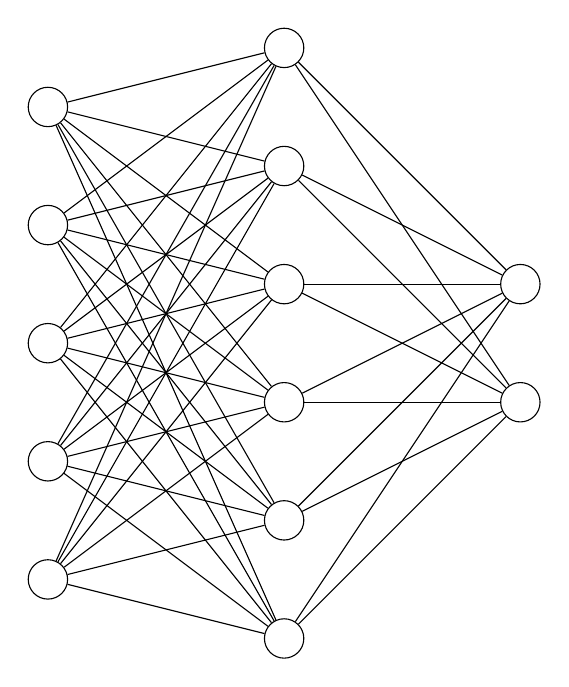
\begin{tikzpicture}
			\foreach \i in {1,...,5} {
					\node[draw, circle, minimum size=0.5cm] (L\i) at (0, -1.5*\i) {};
				}
			\foreach \i in {1,...,6} {
					\node[draw, circle, minimum size=0.5cm] (M\i) at (3, -1.5*\i+0.75) {};
				}
			\foreach \i in {1,...,2} {
					\node[draw, circle, minimum size=0.5cm] (R\i) at (6, -1.5*\i-2.25) {};
				}
			\foreach \i in {1,...,5} {
					\foreach \j in {1,...,6} {
							\draw (L\i) -- (M\j);
						}
				}
			\foreach \i in {1,...,6} {
					\foreach \j in {1,...,2} {
							\draw (M\i) -- (R\j);
						}
				}
		\end{tikzpicture}
	\end{center}
	\caption{Przykładowa wizualizacja trójwartwowej gęstej sieci neuronowej}
	\label{fig:neuron_layers}
\end{figure}

\subsubsection{Sieć neuronowa}

Sieć neuronowa jest rodzajem modelu uczenia maszynowego inspirowanym strukturą biologicznego mózgu. Składa się z neuronów ułożonych w warstwy, które przekształcają dane wejściowe na dane wyjściowe poprzez zestaw połączonych operacji matematycznych.

\paragraph{Struktura sieci:}
Sieć neuronowa składa się z:
\begin{itemize}
	\item \textbf{Warstwy wejściowej:} Przyjmuje surowe dane wejściowe.
	\item \textbf{Warstw ukrytych:} Przetwarzają dane za pomocą neuronów.
	\item \textbf{Warstwy wyjściowej:} Produkuje końcowy wynik.
\end{itemize}

\paragraph{Typy warstw:}
Różne typy warstw stosuje się w zależności od zadania. Poniżej znajduje się tabela przedstawiająca popularne typy warstw:

\begin{table}[!ht]
	\centering
	\caption{Rodzaje warstw w sieciach neuronowych}
	\label{tab:layer_types}
	\begin{center}
		\resizebox{\textwidth}{!}{
			\begin{tabular}{|c|l|}
				\hline
				\textbf{Typ warstwy}                & \textbf{Opis}                                                        \\ \hline
				Gęsta (Fully Connected)             & Każdy neuron jest połączony z każdym neuronem kolejnej warstwy.      \\ \hline
				Konwolucyjna (Convolutional Layer)  & Ekstrakcja cech lokalnych, stosowana w przetwarzaniu obrazów.        \\ \hline
				Rekurencyjna (Recurrent Layer)      & Analiza danych sekwencyjnych, np. tekstu lub szeregów czasowych.     \\ \hline
				Normalizująca (Batch Normalization) & Stabilizacja procesu uczenia poprzez normalizację wejść.             \\ \hline
				Dropout                             & Redukcja nadmiernego dopasowania przez losowe "wyłączanie" neuronów. \\ \hline
			\end{tabular}
		}
	\end{center}
\end{table}

\subsubsection{Neuron}

Neuron jest podstawową jednostką w sieci neuronowej. Otrzymuje dane wejściowe \(x\), które są przekształcane za pomocą wag \(w\) i biasu \(b\) do wartości \(z\):

\[
	z = w \cdot x + b.
\]

Wartość \(z\) jest następnie przekształcana przez funkcję aktywacyjną \(g(z)\), która nadaje sieci nieliniowość.

\subsubsection{Funkcja aktywacyjna}

Funkcja aktywacyjna jest operacją nieliniową stosowaną do wyjść neuronów. Jest kluczowa dla modelowania złożonych zależności w danych.
Może być stosowana w celu wprowadzenia nieliniowych zależności w końcowej warstwie modelu co skutkuje większymi różnicami na wyjściu modelu pomiędzy bliskimi wartościowo neuronami.

\begin{itemize}
	\item{\textbf{ReLU (Rectified Linear Unit):}
	      \[
		      g(z) = \max(0, z).
	      \]
	      \begin{figure}[!ht]
		      \centering
		      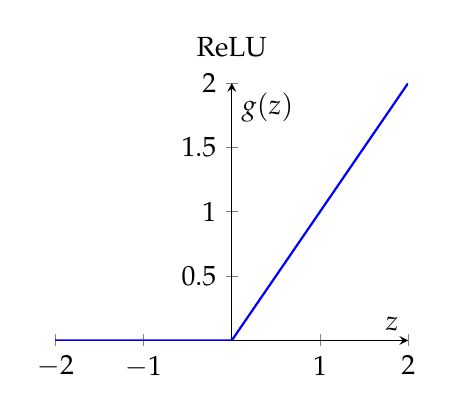
\begin{tikzpicture}
			      \begin{axis}[
					      axis lines=middle,
					      xlabel=$z$,
					      ylabel={$g(z)$},
					      title={ReLU},
					      width=0.5\textwidth,
					      height=0.4\textwidth
				      ]
				      \addplot[domain=-2:2, samples=200, thick, blue] {max(0, x)};
			      \end{axis}
		      \end{tikzpicture}
		      \caption{Funkcja aktywacyjna ReLU.}
		      \label{fig:relu}
	      \end{figure}
	      }
	\item{
	      \textbf{Sigmoid:}
	      \[
		      g(z) = \frac{1}{1 + e^{-z}}.
	      \]
	      \begin{figure}[!ht]
		      \centering
		      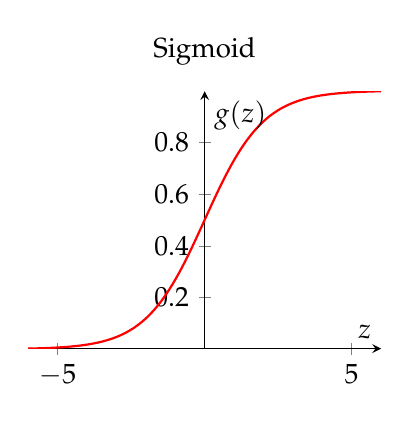
\begin{tikzpicture}
			      \begin{axis}[
					      axis lines=middle,
					      xlabel=$z$,
					      ylabel={$g(z)$},
					      title={Sigmoid},
					      width=0.5\textwidth,
					      height=0.4\textwidth
				      ]
				      \addplot[domain=-6:6, samples=200, thick, red] {1/(1 + exp(-x))};
			      \end{axis}
		      \end{tikzpicture}
		      \caption{Funkcja aktywacyjna Sigmoid.}
		      \label{fig:sigmoid}
	      \end{figure}
	      }
	\item {
	      \textbf{Tanh:}
	      \[
		      g(z) = \tanh(z) = \frac{e^z - e^{-z}}{e^z + e^{-z}}.
	      \]

	      \begin{figure}[!ht]
		      \centering
		      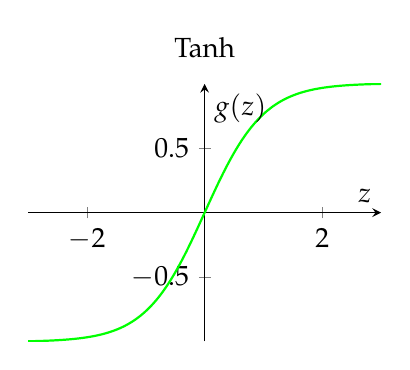
\begin{tikzpicture}
			      \begin{axis}[
					      axis lines=middle,
					      xlabel=$z$,
					      ylabel={$g(z)$},
					      title={Tanh},
					      width=0.5\textwidth,
					      height=0.4\textwidth
				      ]
				      \addplot[domain=-3:3, samples=200, thick, green] {tanh(x)};
			      \end{axis}
		      \end{tikzpicture}
		      \caption{Funkcja aktywacyjna Tanh.}
		      \label{fig:tanh}
	      \end{figure}
	      }
\end{itemize}

\subsubsection{Parametry modelu}

Parametry modelu (np. wagi \(w\) i biasy \(b\)) są wartościami liczbowymi, które model dostosowuje podczas procesu uczenia. Trenowanie modelu polega na minimalizacji funkcji kosztu (ang. loss function), która mierzy różnicę między przewidywaniami modelu a rzeczywistymi wartościami.

%TODO
%\[
%	L = \frac{1}{n} \sum_{i=1}^{n} (y_i - \hat{y}_i)^2,
%\]

gdzie \(y_i\) to rzeczywista wartość, a \(\hat{y}_i\) to przewidywana wartość modelu.

\subsection{Środowisko}
Środowisko jest otoczeniem, w którym agent działa. Dostarcza stanów \( S \), które opisują aktualną sytuację, oraz nagród \( R \), które oceniają jakość podjętych działań.

\begin{itemize}
	\item \textbf{Symulowane gry i światy wirtualne:}
	      \begin{itemize}
		      \item Atari Games (ALE) \cite{BELLEMARE2013}: Gry 8-bitowe, takie jak \textit{Breakout}, \textit{Pong} czy \textit{Space Invaders}.
		      \item Super Mario Bros \cite{KARPATHY2015}: Gra platformowa, w której agent uczy się przechodzić poziomy, omijając przeszkody i eliminując przeciwników.
		      \item OpenAI Gym \cite{BROCKMAN2016}: Zbiór środowisk do testowania algorytmów uczenia ze wzmocnieniem, w tym proste gry i symulacje.
		      \item VizDoom \cite{KEMPKA2016}: Gra FPS (First Person Shooter), gdzie agent eksploruje trójwymiarowe środowisko i uczy się strategii przetrwania.
	      \end{itemize}

	\item \textbf{Środowiska robotyczne:}
	      \begin{itemize}
		      \item MuJoCo \cite{TODOROV2012}: Symulacje robotów do testowania algorytmów sterowania.
		      \item Roboschool \cite{SCHULMAN2017}: Środowiska do trenowania robotów w zadaniach, takich jak chodzenie czy chwytanie obiektów.
		      \item PyBullet \cite{COUMANS2016}: Otwarte środowisko do symulacji fizyki, używane do modelowania zachowań robotów.
	      \end{itemize}

	\item \textbf{Symulacje rzeczywistego świata:}
	      \begin{itemize}
		      \item Autonomous Driving (Carla) \cite{DOSOVITSKIY2017}: Symulacje jazdy autonomicznej.
	      \end{itemize}

	\item \textbf{Środowiska edukacyjne:}
	      \begin{itemize}
		      \item Maze Solvers \cite{SUTTON2018}: Symulacje labiryntów, w których agent uczy się znajdować wyjście.
		      \item GridWorld \cite{RUSSELL2003}: Proste środowisko siatki 2D, gdzie agent uczy się optymalnej strategii poruszania.
	      \end{itemize}
\end{itemize}

\subsection{Stan}

Stan (ang. State) jest kluczowym elementem w uczeniu ze wzmocnieniem, który opisuje bieżącą sytuację w środowisku. Stan zawiera wszystkie istotne informacje potrzebne agentowi do podejmowania decyzji, takich jak pozycja w przestrzeni, otoczenie, zasoby czy inne dane kontekstowe. Formalnie, stan w danym momencie \( t \) oznaczamy jako \( s_t \).

\paragraph{Założenia stanu:}
Stan powinien być na tyle kompletny, aby agent mógł na jego podstawie przewidzieć konsekwencje swoich działań. W praktyce oznacza to, że stan \( s_t \) powinien być wystarczający do określenia następnego stanu \( s_{t+1} \), jeśli znana jest akcja \( a_t \) podjęta przez agenta.

\paragraph{Przykłady stanów w różnych środowiskach:}
Stany mogą przyjmować różne formy w zależności od charakteru środowiska:
\begin{itemize}
	\item \textbf{Gry komputerowe:} W grach wideo stan może obejmować pozycję postaci, punkty życia, liczbę przeciwników oraz przeszkody na planszy. Na przykład w grze Super Mario Bros stan \( s_t \) może zawierać:
	      \begin{itemize}
		      \item Pozycję postaci Mario (\texttt{mario\_x}, \texttt{mario\_y}),
		      \item Liczbę pozostałych żyć,
		      \item Czas do zakończenia poziomu.
	      \end{itemize}
	      Źródło: \cite{BELLEMARE2013, KARPATHY2015}.

	\item \textbf{Robotyka:} W robotyce stan może zawierać:
	      \begin{itemize}
		      \item Kąt wychylenia ramienia robota,
		      \item Pozycję chwytaka,
		      \item Siły oddziałujące na czujniki.
	      \end{itemize}
	      Źródło: \cite{TODOROV2012, SCHULMAN2017}.

	\item \textbf{Autonomiczne pojazdy:} W symulacjach jazdy autonomicznej stan może obejmować:
	      \begin{itemize}
		      \item Pozycję pojazdu względem pasa ruchu,
		      \item Prędkość i przyspieszenie,
		      \item Pozycję innych pojazdów oraz sygnalizację świetlną.
	      \end{itemize}
	      Źródło: \cite{DOSOVITSKIY2017}.
\end{itemize}

\paragraph{Reprezentacja stanu:}
Stan może być reprezentowany w różnych formatach w zależności od charakteru środowiska:
\begin{itemize}
	\item Wartości liczbowe (np. pozycja na planszy),
	\item Macierze (np. obrazy w grach komputerowych),
	\item Grafy (np. w symulacjach sieci społecznych lub ruchu drogowego).
\end{itemize}

\paragraph{Wymagania wobec stanu:}
Aby algorytm mógł skutecznie działać, stan powinien być:
\begin{itemize}
	\item \textbf{Dostępny:} Agent musi być w stanie zaobserwować stan \( s_t \) w każdym kroku czasowym \( t \).
	\item \textbf{Markowski:} Stan \( s_t \) musi być kompletny, tj. zawierać wszystkie informacje potrzebne do określenia przyszłości na podstawie bieżących akcji (\emph{Markov Decision Process}\cite{PUTERMAN1994}).
\end{itemize}

\paragraph{Znaczenie stanu w uczeniu ze wzmocnieniem:}
Dokładne określenie stanu jest kluczowe dla skuteczności algorytmu. Niekompletny lub zbyt uproszczony stan może prowadzić do nieoptymalnych decyzji agenta, natomiast nadmiarowa ilość informacji w stanie zwiększa złożoność obliczeniową algorytmu.

\paragraph{Wpływ na złożoność obliczeniową:}
Ilość parametrów modelu (wagi i biasy) rośnie wraz z liczbą połączeń neuronów. W przypadku wielowarstwowych sieci neuronowych liczba parametrów gwałtownie wzrasta, co prowadzi do większych wymagań obliczeniowych i pamięciowych. Dla warstwy gęstej (ang. fully connected) liczba parametrów \(P\) jest określana jako:

\[
	P = (n_{\text{input}} \cdot n_{\text{output}}) + n_{\text{output}},
\]

gdzie:
\begin{itemize}
	\item \(n_{\text{input}}\) – liczba neuronów wejściowych,
	\item \(n_{\text{output}}\) – liczba neuronów wyjściowych,
	\item \(n_{\text{output}}\) dodatkowo uwzględnia biasy.
\end{itemize}

Zwiększanie liczby warstw i neuronów pozwala na modelowanie bardziej złożonych funkcji, ale także zwiększa ryzyko nadmiernego dopasowania (ang. overfitting) oraz wydłuża czas trenowania modelu. Optymalizacja liczby parametrów jest kluczowa dla zachowania równowagi między dokładnością modelu a jego efektywnością obliczeniową.

\subsection{Akcja}

Akcja (ang. Action) to decyzja podejmowana przez agenta w danym stanie środowiska. Określa, jak agent wpływa na otoczenie, prowadząc do zmiany stanu i potencjalnego otrzymania nagrody. Zbiór wszystkich możliwych akcji agenta nazywa się przestrzenią akcji \(A\).

\paragraph{Typy przestrzeni akcji:}
\begin{itemize}
	\item \textbf{Skończona (ang. Discrete):} Agent wybiera spośród ograniczonej liczby akcji, np. ruch w lewo, w prawo, skok.
	\item \textbf{Ciągła (ang. Continuous):} Agent wybiera wartość z określonego przedziału, np. prędkość czy kąt obrotu.
\end{itemize}

\paragraph{Przykłady akcji:}
\begin{itemize}
	\item Ruch przestrzenny, np. zmiana pozycji w labiryncie.
	\item Manipulacja obiektami, np. podnoszenie lub przesuwanie przedmiotów.
	\item Regulacja parametrów, np. ustawianie prędkości w pojazdach autonomicznych.
\end{itemize}

Każda akcja prowadzi do zmiany stanu środowiska \(s_t\) na \(s_{t+1}\), zgodnie z funkcją przejścia \(P(s_{t+1} | s_t, a_t)\). Wybór akcji jest określany przez strategię (ang. policy), która może być deterministyczna lub stochastyczna.

\subsection{Nagroda}

Nagroda (ang. Reward) to wartość liczbowa, którą agent otrzymuje po wykonaniu akcji w danym stanie. Jest kluczowym elementem w uczeniu ze wzmocnieniem, ponieważ kieruje zachowaniem agenta, motywując go do podejmowania działań prowadzących do maksymalizacji długoterminowych korzyści. Nagroda w danym kroku czasowym \(t\) oznaczana jest jako \(r_t\).

\paragraph{Dobór funkcji nagrody:}
Projektowanie funkcji nagrody wymaga ostrożności, ponieważ niewłaściwy dobór może prowadzić do niepożądanego zachowania agenta. Dobrze zaprojektowana funkcja nagrody powinna:
\begin{itemize}
	\item Być zgodna z celem środowiska (np. szybkie ukończenie zadania, minimalizacja kosztów).
	\item Karać za niepożądane działania (np. kolizje w robotyce, utratę życia w grze).
	\item Oferować natychmiastową informację zwrotną, aby przyspieszyć proces uczenia.
\end{itemize}

\paragraph{Normalizacja nagrody:}
Normalizacja nagrody polega na skalowaniu wartości \(r_t\) do określonego zakresu, np. \([-1, 1]\), co zapobiega dominacji ekstremalnych wartości nad procesem uczenia. Może to również pomóc w stabilizacji algorytmu i przyspieszeniu zbieżności. Typowe metody normalizacji to:
\begin{itemize}
	\item \textbf{Z-score normalization:} Skalowanie względem średniej i odchylenia standardowego:
	      \[
		      r_t' = \frac{r_t - \mu_r}{\sigma_r},
	      \]
	      gdzie \(\mu_r\) i \(\sigma_r\) są odpowiednio średnią i odchyleniem standardowym nagród.
	\item \textbf{Min-max scaling:} Skalowanie do określonego zakresu:
	      \[
		      r_t' = \frac{r_t - \min(r)}{\max(r) - \min(r)}.
	      \]
\end{itemize}

\paragraph{Przykłady nagród:}
\begin{itemize}
	\item W grach komputerowych: zdobycie punktów, przejście na kolejny poziom, kara za utratę życia \cite{BELLEMARE2013}.
	\item W robotyce: nagroda za poprawne uchwycenie przedmiotu lub utrzymanie równowagi \cite{TODOROV2012}.
	\item W pojazdach autonomicznych: nagroda za płynne poruszanie się po drodze, kara za kolizje \cite{DOSOVITSKIY2017}.
\end{itemize}

\subsection{Funkcja kosztu (Loss)}

Funkcja kosztu jest kluczowym elementem procesu uczenia modelu, ponieważ określa, jak bardzo bieżące predykcje modelu różnią się od wartości docelowych. W przypadku uczenia ze wzmocnieniem (ang. Reinforcement Learning), funkcja kosztu jest związana z różnicą pomiędzy bieżącymi wartościami \(Q(s, a)\) a wartościami docelowymi wyznaczonymi na podstawie nagród i przewidywań przyszłych stanów.

\paragraph{Znaczenie funkcji kosztu:}
\begin{itemize}
	\item \textbf{Minimalizacja różnic:} Funkcja kosztu prowadzi do optymalizacji parametrów modelu \(\theta\), minimalizując różnice pomiędzy bieżącymi wartościami \(Q(s, a)\) a wartościami docelowymi.
	\item \textbf{Stabilność procesu uczenia:} Wprowadzenie sieci docelowej \(\theta^{-}\) pozwala na bardziej stabilne obliczanie wartości docelowych \(y_t\), co zapobiega niestabilności procesu uczenia wynikającej z dynamicznie zmieniających się wartości \(Q(s, a)\).
	\item \textbf{Wrażliwość na parametry:} Funkcja kosztu jest wrażliwa na odpowiedni dobór współczynnika dyskontowego \(\gamma\) i strategii aktualizacji sieci docelowej, co wpływa na szybkość i jakość uczenia.
\end{itemize}

\section{Double Q-Learning}

Double Q-Learning to zaawansowany algorytm uczenia ze wzmocnieniem, będący rozszerzeniem klasycznego Q-Learningu. Jego głównym celem jest redukcja przeszacowania wartości akcji, co jest typowym problemem w tradycyjnym Q-Learningu. W tej sekcji omówione zostaną podstawy algorytmu Q-Learning, problem przeszacowania, struktura Double Q-Learning oraz jego zastosowania.

\subsection{Podstawy Q-Learning}

Q-Learning jest jednym z najbardziej znanych algorytmów uczenia ze wzmocnieniem, który pozwala agentowi uczyć się optymalnej strategii działania w środowisku poprzez iteracyjne aktualizowanie funkcji wartości \(Q(s, a)\). Funkcja ta ocenia korzyść z podjęcia określonej akcji \(a\) w stanie \(s\).

Równanie aktualizacji w klasycznym Q-Learningu opiera się na równaniu Bellmana:

\begin{equation}Q(s, a) \leftarrow Q(s, a) + \alpha \left( r + \gamma \max_{a'} Q(s', a') - Q(s, a) \right)\end{equation}

gdzie:
\begin{itemize}
	\item \(s\) – aktualny stan,
	\item \(a\) – podjęta akcja,
	\item \(r\) – nagroda za wykonanie akcji \(a\),
	\item \(s'\) – następny stan po wykonaniu akcji \(a\),
	\item \(\alpha\) – współczynnik uczenia, kontrolujący szybkość aktualizacji,
	\item \(\gamma\) – współczynnik dyskontowy, określający znaczenie przyszłych nagród.
\end{itemize}

Celem algorytmu Q-Learning jest iteracyjne zbliżanie wartości funkcji \(Q(s, a)\) do jej optymalnych wartości \(Q^*(s, a)\). Wartość \(Q^*(s, a)\) reprezentuje maksymalną sumę oczekiwanych nagród, jaką agent może uzyskać, rozpoczynając w stanie \(s\), wykonując akcję \(a\), a następnie postępując zgodnie z najlepszą możliwą strategią.

\subsection{Problem przeszacowania wartości}

W Q-Learningu akcje są wybierane na podstawie maksymalnej wartości \(Q(s, a)\). Jednak proces aktualizacji również wykorzystuje tę maksymalną wartość, co prowadzi do przeszacowania wyników, szczególnie w środowiskach o dużej zmienności. Problem przeszacowania wynika z faktu, że maksymalizowanie wartości \(Q(s, a)\) na etapie wyboru i aktualizacji wprowadza błędy, które się kumulują.

\subsection{Double Q-Learning: Struktura i działanie}

Double Q-Learning rozwiązuje problem przeszacowania, wprowadzając dwie oddzielne funkcje wartości, \(Q_1\) i \(Q_2\). Te funkcje są aktualizowane naprzemiennie, co pozwala na rozdzielenie procesu wyboru akcji od procesu aktualizacji wartości.

\paragraph{Równania aktualizacji:}
W danym kroku czasowym \(t\):
\begin{itemize}
	\item Jeśli aktualizowana jest funkcja \(Q_1\), proces przebiega według wzoru:
	      \begin{equation}Q_1(s, a) \leftarrow Q_1(s, a) + \alpha \left( r + \gamma Q_2(s', \arg\max_{a'} Q_1(s', a')) - Q_1(s, a) \right)\end{equation}
	\item Jeśli aktualizowana jest funkcja \(Q_2\), proces przebiega według wzoru:
	      \begin{equation}Q_2(s, a) \leftarrow Q_2(s, a) + \alpha \left( r + \gamma Q_1(s', \arg\max_{a'} Q_2(s', a')) - Q_2(s, a) \right)\end{equation}
\end{itemize}

Rozdzielenie aktualizacji między \(Q_1\) i \(Q_2\) pozwala na bardziej precyzyjne oszacowanie wartości \(Q(s, a)\), ponieważ wybór akcji opiera się na jednej funkcji, a aktualizacja na drugiej.

\paragraph{Strategia \(\epsilon\)-greedy}

Strategia \(\epsilon\)-greedy (ang. \(\epsilon\)-greedy policy) to jedna z najczęściej stosowanych metod równoważenia eksploracji i eksploatacji w uczeniu ze wzmocnieniem. Celem tej strategii jest umożliwienie agentowi eksploracji środowiska (odkrywanie nowych akcji) przy jednoczesnym wykorzystywaniu najlepszych dotychczasowych decyzji.

W strategii \(\epsilon\)-greedy agent wybiera akcję w następujący sposób:
\begin{itemize}
	\item Z prawdopodobieństwem \(1 - \epsilon\) wybiera akcję o najwyższej wartości \(Q(s, a)\), czyli eksploatuje dotychczasową wiedzę.
	\item Z prawdopodobieństwem \(\epsilon\) wybiera losową akcję, eksplorując nowe możliwości.
\end{itemize}

Parametr \(\epsilon \in [0, 1]\) kontroluje równowagę między eksploracją a eksploatacją:
\begin{itemize}
	\item Dla \(\epsilon = 0\) agent zawsze wybiera akcję o maksymalnej wartości \(Q(s, a)\), całkowicie eksploatując swoją wiedzę.
	\item Dla \(\epsilon = 1\) agent zawsze wybiera losową akcję, skupiając się wyłącznie na eksploracji.
\end{itemize}

Często stosuje się harmonogram zmiany wartości \(\epsilon\) w czasie, tzw. \textit{annealing}, gdzie \(\epsilon\) początkowo jest wysokie (intensywna eksploracja), a następnie maleje w miarę zdobywania przez agenta wiedzy o środowisku. Dzięki temu na początku agent może zbierać informacje o środowisku, a później optymalizować swoje działania na podstawie dotychczasowych doświadczeń.

\paragraph{Model online i model docelowy}

W Double Q-Learning algorytm opiera się na rozdzieleniu funkcji wartości \(Q\) na dwie oddzielne funkcje: model online i model docelowy (ang. target model). Takie podejście pozwala na większą stabilność uczenia i bardziej precyzyjne oszacowanie wartości \(Q(s, a)\).

\begin{itemize}
	\item \textbf{Model online:} Jest to główny model używany do podejmowania decyzji przez agenta. Na podstawie modelu online agent wybiera akcje w danym stanie \(s\), kierując się strategią \( \epsilon\)-greedy lub inną strategią eksploracyjno-eksploatacyjną.
	\item \textbf{Model docelowy (target model):} Służy do aktualizacji wartości docelowych w procesie uczenia. Model docelowy jest kopią modelu online, aktualizowaną w regularnych odstępach czasu, co zapobiega nadmiernym oscylacjom wartości \(Q\) i poprawia stabilność algorytmu.
\end{itemize}

Aktualizacja wartości \(Q\) w Double Q-Learning wykorzystuje obydwa modele:
\begin{itemize}
	\item Model online wybiera najlepszą akcję w stanie \(s'\), tj. \(\arg\max_{a'} Q_\text{online}(s', a')\).
	\item Model docelowy dostarcza wartość \(Q\) dla wybranej akcji:
	      \begin{equation}Q_\text{target}(s, a) \leftarrow r + \gamma Q_\text{online}(s', \arg\max_{a'} Q_\text{target}(s', a')).\end{equation}
\end{itemize}

Rozdzielenie wyboru akcji i ich aktualizacji na dwa modele redukuje ryzyko przeszacowania, ponieważ proces wyboru akcji i oceny ich wartości odbywa się w niezależnych kopiach funkcji \(Q\).

\subsection{Funkcja kosztu w Double Q-Learning:}

Dla algorytmu Double Q-Learning, funkcja kosztu jest definiowana jako błąd średniokwadratowy (ang. Mean Squared Error, MSE) pomiędzy wartością docelową \(y_t\) a bieżącą wartością \(Q(s_t, a_t)\):

\begin{equation}L(\theta) = \mathbb{E}_{s_t, a_t, r_t, s_{t+1}} \left[ \left( y_t - Q(s_t, a_t; \theta) \right)^2 \right],\end{equation}
gdzie:
\begin{itemize}
	\item \(y_t = r_t + \gamma Q(s_{t+1}, \arg\max_a Q(s_{t+1}, a; \theta); \theta^{-})\) – wartość docelowa wyznaczona przy użyciu sieci docelowej \(\theta^{-}\).
	\item \(\gamma\) – współczynnik dyskontowy, który określa wpływ przyszłych nagród.
	\item \(r_t\) – nagroda uzyskana w bieżącym kroku.
\end{itemize}

\subsection{Zalety Double Q-Learning}

Double Q-Learning ma kilka istotnych zalet w porównaniu z klasycznym Q-Learningiem:
\begin{itemize}
	\item \textbf{Redukcja przeszacowania:} Rozdzielenie procesu wyboru i aktualizacji wartości zmniejsza ryzyko błędów wynikających z nadmiernej optymistycznej oceny.
	\item \textbf{Lepsza stabilność:} Algorytm działa bardziej przewidywalnie w środowiskach o dużej zmienności lub hałasie.
	\item \textbf{Elastyczność:} Double Q-Learning można łatwo rozszerzyć na bardziej złożone algorytmy, takie jak Deep Q-Learning.
\end{itemize}

\chapter{Projekt systemu}
\begin{figure}[ht]
	\begin{center}
		\resizebox{\textwidth}{!}{
			\begin{tikzpicture}[
					node distance=2.5cm, % Odstęp między węzłami
					align=center, % Wyśrodkowanie tekstu w węzłach
					>=latex, % Strzałki w stylu LaTeX
					%every node/.style={draw, text width=3cm} % Styl węzłów
				]

				\node[rectangle, minimum width=5cm, draw=black] (full_frame) {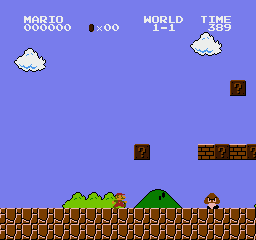
\includegraphics[width=4cm]{img/full_frame.png}\\Obraz generowany przez emulator NES};

				\node[right of=full_frame, xshift=6cm, draw=black] (compressed_frame) {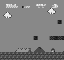
\includegraphics[width=2.5cm]{img/compressed_frame.png} \\Skompresowany obraz};
				\node (model) [right of=compressed_frame, draw = black, minimum height=2cm, xshift=2cm] {Model};
				\node (controller) [right of=model, draw=black, minimum height = 2cm, xshift=1cm, minimum width = 2cm] {Przyciski\\kontrolera\\NES};

				\draw[<-] (compressed_frame.west) -- (full_frame.east) node[midway] {Zmniejszenie\\ rozmiaru i \\ konwersja na skalę \\szarości};
				\draw[<-] (model.west) -- (compressed_frame.east) node[midway]{Konwersja\\na tensor};
				\draw[<-] (controller.west) -- (model.east) node[midway] {Predykcja\\wciśnięć};

			\end{tikzpicture}
		}
	\end{center}
	\caption{Ogólny schemat działania programu}
	\label{fig:sys_diagram}
\end{figure}

\chapter{Implementacja}

Implementacja projektu została zrealizowana przy użyciu kilku kluczowych technologii i narzędzi wspierających proces uczenia modelu oraz monitorowanie eksperymentów. Poniżej przedstawiono najważniejsze szczegóły implementacyjne oraz architekturę systemu.

\section{Technologie}

\begin{itemize}
	\item \textbf{PyTorch:} Biblioteka do budowy i trenowania modelu DQN (Deep Q-Network) oraz implementacji warstw konwolucyjnych, w pełni połączonych i mechanizmów propagacji gradientów.
	\item \textbf{Weights and Biases (WandB):} Narzędzie do monitorowania eksperymentów, umożliwiające śledzenie hiperparametrów, wyników oraz wizualizację metryk uczenia.
	\item \textbf{Własny algorytm DQN:} Algorytm Double Q-Learning został zaimplementowany ręcznie w celu lepszego dostosowania do specyficznych wymagań projektu.
\end{itemize}
\section{Architektura systemu}

Cały system został zaprojektowany do pracy na zdalnej maszynie wyposażonej w GPU NVIDIA, gdzie jednocześnie działa wiele procesów związanych z różnymi modelami. System korzysta z dodatkowych narzędzi, takich jak \texttt{WandB} do monitorowania i archiwizacji oraz \texttt{SQLite} do przechowywania parametrów modelu i stanu optymalizatora. Architektura systemu jest przedstawiona na rysunku~\ref{fig:systemarchitecture}.

\begin{figure}[!ht]
	\begin{center}
		\resizebox{1\textwidth}{!}{%
			\begin{circuitikz}
				\tikzstyle{every node}=[font=\small]
				\draw  (6,10.5) rectangle (4,12.5);
				\draw [ dashed] (2.75,7.5) rectangle  (6.75,13.75);
				\draw [ fill={rgb,255:red,255; green,255; blue,255} ] (5.75,10.75) rectangle (3.75,12.75);
				\draw [ fill={rgb,255:red,255; green,255; blue,255} ] (5.5,11) rectangle  node {\scriptsize Procesy trenujące} (3.5,13);
				\draw [ fill={rgb,255:red,255; green,255; blue,255} , dashed] (3.75,11.25) rectangle  node {\footnotesize Model}  (5.25,11.75);
				\node [font=\small] at (4,13.5) {};
				\node [font=\small] at (4.75,13.5) {Zdalna maszyna GPU};
				\draw  (4,9.75) rectangle  node {\scriptsize Baza danych} (5.5,8.25);
				\draw  (-2.25,12.75) rectangle  node {\small WandB} (0,8.25);
				\draw [<->, >=Stealth] (4.75,9.75) -- (4.75,10.5)node[pos=0.5, fill=white, font=\footnotesize]{Zapisywanie modeli};
				\draw [->, >=Stealth] (3.5,12) -- (0,12)node[pos=0.5, fill=white, font=\scriptsize]{Agregacja danych};
			\end{circuitikz}
		}
	\end{center}
	\caption{Architektura systemu}
	\label{fig:systemarchitecture}
\end{figure}

\begin{itemize}
	\item \textbf{Zdalna maszyna z GPU:} System działa na serwerze wyposażonym w GPU NVIDIA, umożliwiając równoczesne trenowanie kilku modeli. GPU przydzielane są do poszczególnych procesów w zależności od obciążenia.
	\item \textbf{Weights and Biases (WandB):} WandB jest używane do monitorowania eksperymentów. Zapisuje logi, metryki (np. stratę i nagrody) oraz regularnie archiwizuje stany modelu i optymalizatora.
	\item \textbf{SQLite:} Lekka baza danych SQLite przechowuje parametry modelu, stany optymalizatora oraz inne dane konfiguracyjne, co umożliwia łatwe wznowienie treningu lub analizę po zakończeniu procesu.
	\item \textbf{Archiwum modeli:} Modele i stany optymalizatora są regularnie zapisywane w formacie binarnym w lokalnym archiwum, co pozwala na późniejsze wykorzystanie i ewaluację.
	\item \textbf{Procesy równoległe:} Na maszynie uruchamiane są równocześnie różne procesy, z których każdy zajmuje się trenowaniem innego modelu. WandB synchronizuje dane z każdego procesu w czasie rzeczywistym.
\end{itemize}

\section{Monitorowanie i archiwizacja}

Dzięki integracji z WandB i SQLite proces treningu jest w pełni monitorowany. WandB umożliwia wizualizację wyników w czasie rzeczywistym, a SQLite zapewnia
\section{Uruchomienie systemu}

System działa na zdalnej maszynie, co wymaga:
\begin{itemize}
	\item Konfiguracji środowiska wirtualnego z bibliotekami \texttt{PyTorch}, \texttt{WandB} oraz dodatkowymi zależnościami.
	\item Połączenia z serwerem WandB w celu monitorowania eksperymentów.
	\item Uruchomienia emulatora NES i algorytmu DQN na zdalnej maszynie wyposażonej w GPU.
\end{itemize}

Proces treningu obejmuje iteracyjne aktualizowanie modelu DQN, przesyłanie wyników do WandB oraz przechowywanie danych w Replay Buffer w celu stabilizacji procesu uczenia.

\chapter{Eksperymenty i wyniki}

W tym rozdziale zaprezentowano wyniki przeprowadzonych eksperymentów oraz ich analizę. Skupiono się na ocenie najlepszego modelu, wpływie parametrów treningowych  oraz funkcji nagrody na proces uczenia i końcowe wyniki agenta.

\section{Wyniki najlepszego modelu}

Najlepszy model został wybrany na podstawie maksymalnej średniej nagrody.

\begin{figure}[!ht]
	\centering
	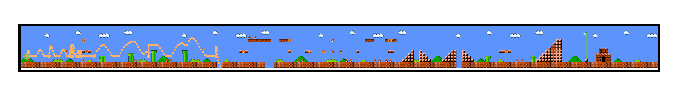
\includegraphics[width=\textwidth]{plots/pos.eps}
	\caption{Wyniki najlepszego modelu: pozycja agenta naniesiona na mapę poziomu\(x_{\text{pos}}\).}
	\label{fig:best_model_results}
\end{figure}

Model osiągnął maksymalną pozycję \(x_{\text{pos}}\) wynoszącą \(1151\) (około \(\frac{1}{3}\) poziomu) oraz średnią nagrodę \(127.718\) na epizod po 2560 epizodach.

\section{Proces trenowania}

Podczas trenowania modelu agent stopniowo uczył się strategii pozwalających na skuteczniejsze poruszanie się po poziomie w grze \textit{Super Mario Bros}. Na rysunku~\ref{fig:training_process} przedstawiono wykres ilustrujący maksymalną osiągniętą pozycję \(x_{\text{pos}}\) w funkcji liczby epizodów.

\begin{figure}[!ht]
	\centering
	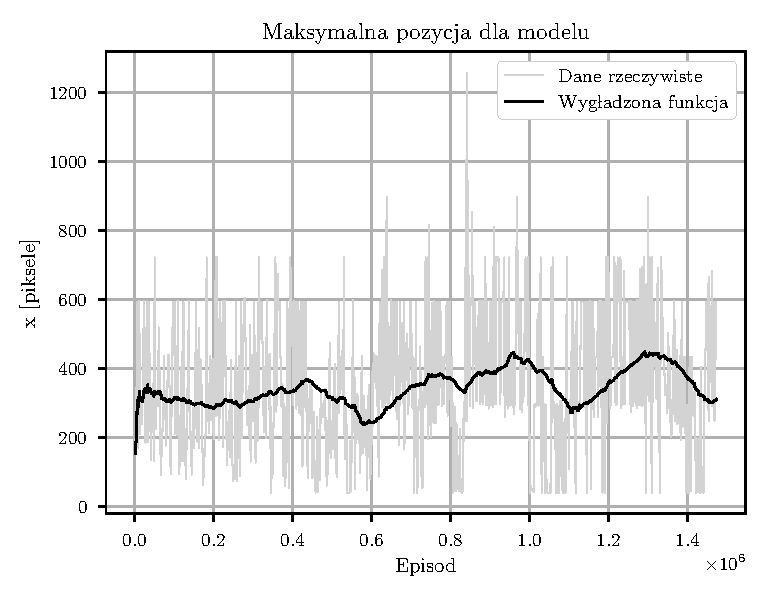
\includegraphics[width=0.8\textwidth]{plots/max_x.eps}
	%\includegraphics[width=0.8\textwidth]{training_process.png}
	\caption{Proces trenowania: maksymalna pozycja \(x_{\text{pos}}\) w zależności od liczby epizodów.}
	\label{fig:training_process}
\end{figure}

\paragraph{Wnioski:}

Wzrost wartości \(x_{\text{pos}}\) w trakcie trenowania nie jest liniowy, co jest wynikiem złożoności środowiska oraz charakterystyki procesu uczenia:
\begin{itemize}
	\item \textbf{Złożoność środowiska gry:} W grze agent napotyka różnorodne przeszkody i przeciwników, które wpływają na jego zachowanie. W niektórych epizodach agent może trafić na sytuacje, których wcześniej nie doświadczył, co prowadzi do spadku wyników.
	\item \textbf{Duża przestrzeń wejściowa:} Relatywnie wysoka liczba pikseli w obrazie wejściowym (\(60 \times 64\)) powoduje, że model musi analizować znaczną ilość informacji, co utrudnia szybkie generowanie optymalnych strategii.
	\item \textbf{Eksploracja i eksploatacja:} Strategia \(\epsilon\)-greedy sprawia, że w początkowych etapach agent częściej eksploruje nowe akcje, co prowadzi do spadku wyników w epizodach, gdzie nowe strategie okazują się nieskuteczne.
	\item \textbf{Dynamiczny charakter nagród:} Model jest nagradzany za różnorodne aspekty gry (prędkość, postęp, eliminację przeciwników). Równoczesna optymalizacja wielu składników funkcji nagrody może prowadzić do okresowych spadków wyników, gdy agent próbuje dostosować swoje działania.
\end{itemize}

Pomimo tych trudności, ogólny trend wskazuje na stały wzrost wartości \(x_{\text{pos}}\) w dłuższym okresie. Spadki są naturalnym elementem procesu uczenia w złożonych środowiskach, ponieważ agent dostosowuje swoje strategie do coraz bardziej wymagających sytuacji w grze.

\section{Porównanie różnych wartości wygaszania \(\epsilon\)}

Eksperymenty przeprowadzono dla trzech różnych schematów wygaszania \(\epsilon\):
\begin{itemize}
	\item \textbf{Za szybkie wygaszanie:} Początkowe \(\epsilon = 1.0, \epsilon_d=0.95\), wygaszanie w \(76\) krokach.
	\item \textbf{Optymalne wygaszanie:} Początkowe \(\epsilon = 1.0, \epsilon_d=0.994\), wygaszanie w \(765\) krokach.
	\item \textbf{Za wolne wygaszanie:} Początkowe \(\epsilon = 1.0, \epsilon_d=0.997\), wygaszanie w \(1500\) krokach.
\end{itemize}

Na rysunku~\ref{fig:epsilon_comparison} przedstawiono wpływ różnych schematów na średnią nagrodę oraz wartość funkcji kosztu.

\begin{figure}[!ht]
	\centering
	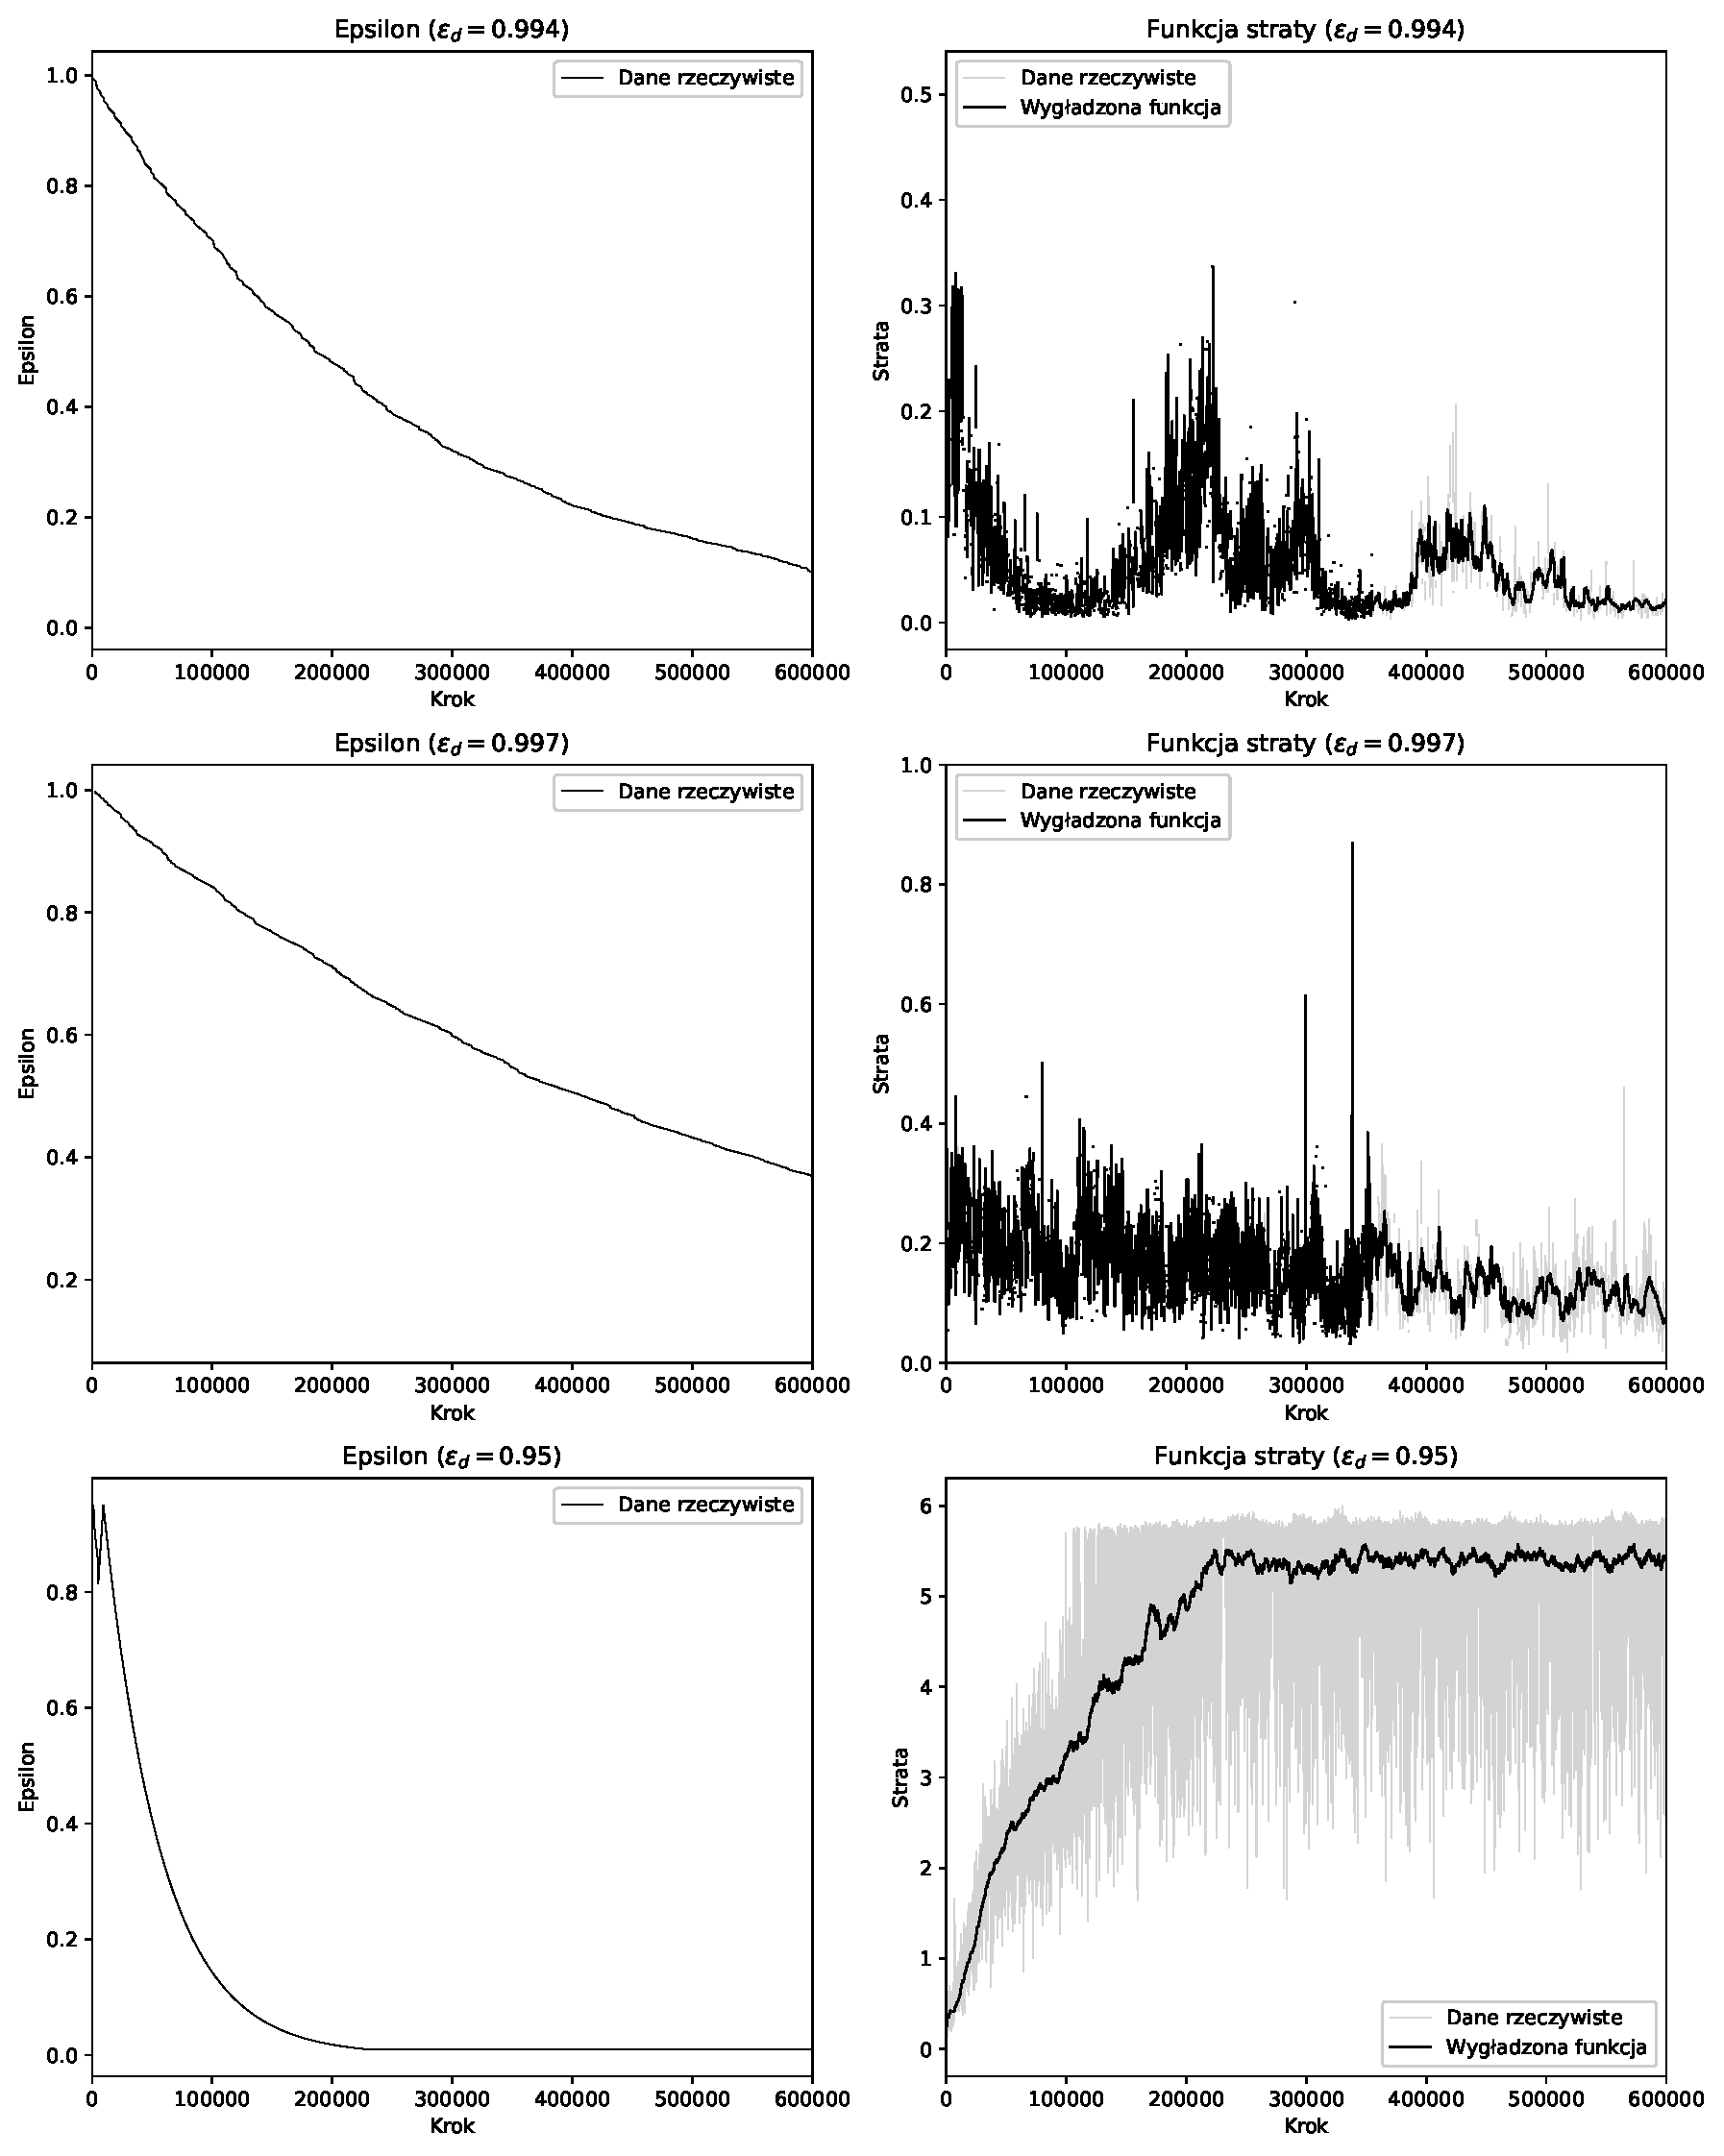
\includegraphics[width=\textwidth]{plots/epsilon.eps}
	\caption{Porównanie wpływu różnych schematów \(\epsilon\) na nagrodę (lewy wykres) i stratę (prawy wykres).}
	\label{fig:epsilon_comparison}
\end{figure}

\paragraph{Wnioski:}
Zbyt szybkie wygaszanie powodowało, że agent nie nadążał z eksploracją, co prowadziło do wysokiej wartości funkcji kosztu, która nie wracała do niższych wartości. Z kolei zbyt wolne wygaszanie znacząco wydłużyło czas uczenia. Model ze zbyt szybkim wygaszaniem \(\epsilon\) niedostatecznie zeksplorował własne środowisko i ostatecznie nie dokonał żadnych zmian co do rezultatów.

\section{Wpływ funkcji nagrody}

Eksperymenty dotyczyły modyfikacji funkcji nagrody poprzez manipulację wagami nagrody za prędkość (\texttt{speed}) i pozycję (\texttt{position\_reward}). Na rysunku~\ref{fig:reward_comparison} przedstawiono maksymalne wartości \(x_{\text{pos}}\) dla różnych konfiguracji.

\begin{figure}[!ht]
	\centering
	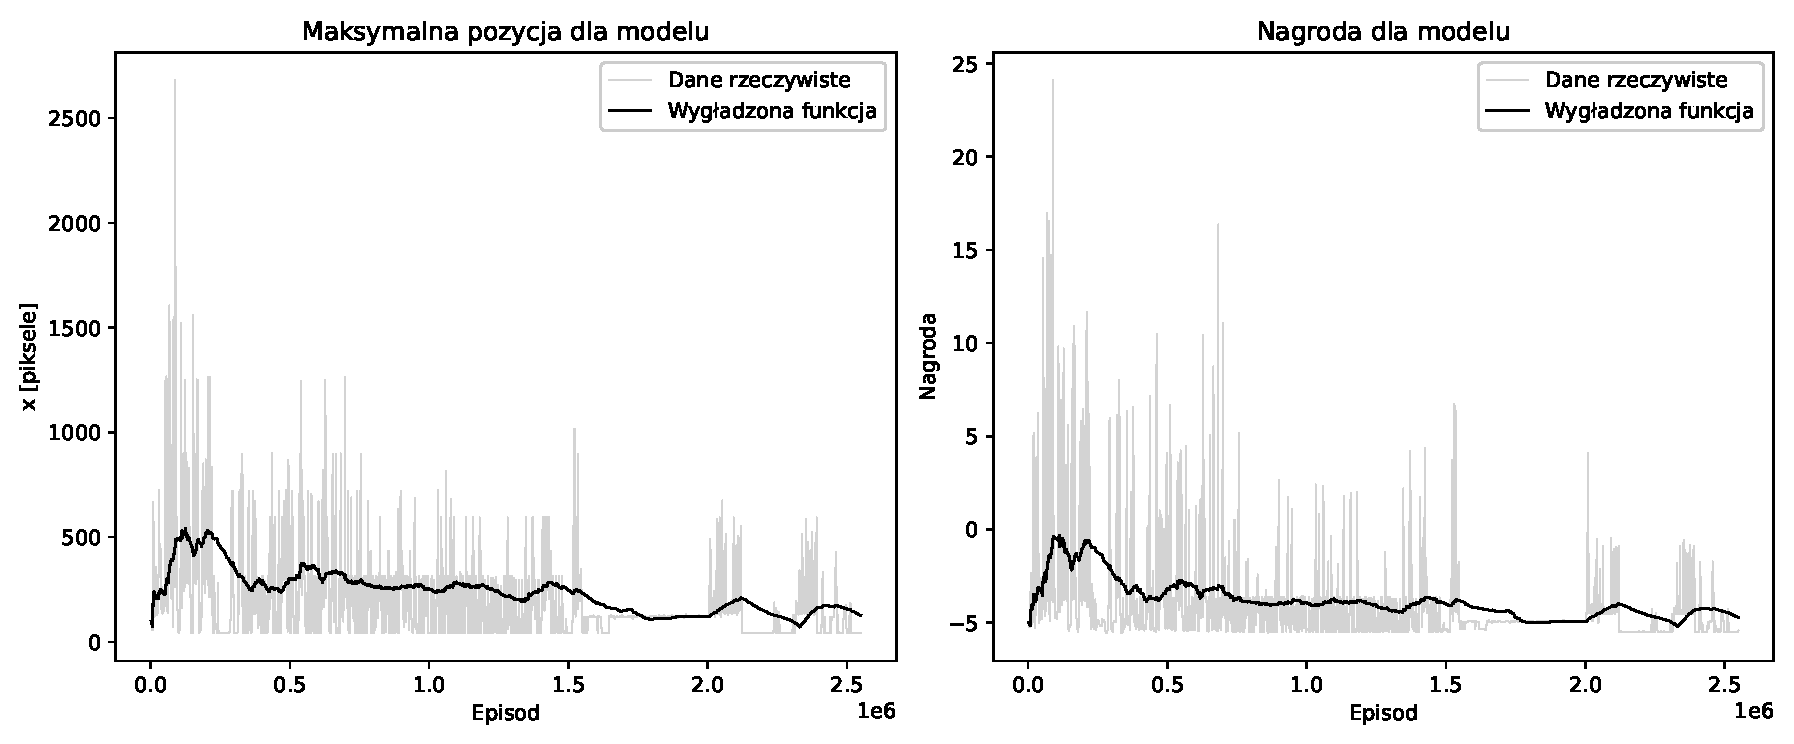
\includegraphics[width=\textwidth]{plots/reward.eps}
	%\includegraphics[width=0.8\textwidth]{reward_function_comparison.png}
	\caption{Wpływ funkcji nagrody na maksymalną pozycję \(x_{\text{pos}}\).}
	\label{fig:reward_comparison}
\end{figure}
\paragraph{Wnioski:}

Eksperymenty wykazały, że niewłaściwy dobór funkcji nagrody znacząco wpływa na skuteczność procesu uczenia. Jeśli nagroda była skoncentrowana wyłącznie na pozycji \(x_{\text{pos}}\), agent priorytetowo traktował poruszanie się w poziomie, ignorując inne aspekty gry, takie jak unikanie przeciwników czy eksploracja otoczenia. Prowadziło to do sytuacji, w której model uczył się niskiej jakości strategii, szybko osiągając maksymalne wartości nagrody, ale z pominięciem ważnych elementów gry.

Z kolei zbyt wysokie kary, takie jak te wynikające z dużych wartości ujemnych za śmierć lub przekroczenie czasu, skutkowały spadkiem stabilności procesu uczenia. Agent unikał eksploracji, obawiając się wysokich strat, co prowadziło do lokalnych minimów w funkcji wartości \(Q(s, a)\). W rezultacie model nie potrafił poprawnie uczyć się złożonych strategii, a maksymalne wartości \(x_{\text{pos}}\) osiągane w trakcie treningu były znacznie niższe.

Optymalne wyniki uzyskano, gdy funkcja nagrody była dobrze zbalansowana — uwzględniała zarówno postęp w poziomie (\(x_{\text{pos}}\)), jak i inne kluczowe aspekty, takie jak prędkość czy unikanie ryzyka. Takie podejście pozwoliło agentowi na bardziej zrównoważony rozwój strategii, co przełożyło się na wyższe wartości \(x_{\text{pos}}\) oraz stabilniejszy proces uczenia.

\section{Podsumowanie wyników}

Eksperymenty wykazały, że:
\begin{itemize}
	\item Optymalne wygaszanie \(\epsilon\) oraz \(\gamma = 0.994\) zapewniały stabilny proces uczenia.
	\item Manipulacja funkcją nagrody pozwalała na dostosowanie zachowania agenta, ale wymagała równowagi między różnymi składnikami nagrody.
\end{itemize}

\chapter[Przegląd literatury]{PrzeglĄd literatury}
\label{chap:przeglad}
Uczenie ze wzmocnieniem (ang. Reinforcement Learning, RL) jest jednym z najważniejszych podejść do sztucznej inteligencji, szczególnie w kontekście sterowania agentami w złożonych środowiskach, takich jak gry wideo. W literaturze naukowej można znaleźć liczne prace badające różne aspekty i ulepszenia algorytmów RL, które w znaczący sposób przyczyniły się do rozwoju tej dziedziny. W szczególności, prace poświęcone grze Super Mario Bros oraz innym platformom do gier, takim jak Atari czy Nintendo Entertainment System (NES), pozwalają lepiej zrozumieć wyzwania stojące przed algorytmami RL.

W pracy LeBlanca i Lee \cite{NES} autorzy badali zastosowanie uczenia ze wzmocnieniem wśrodowisku konsoli do gier NES. Autorzy wykorzystali agentów RL, którzy byli trenowani bez dostarczania wiedzy eksperckiej, co pozwoliło na zbadanie, jak dobrze nowoczesne algorytmy są w stanie sobie radzić w środowiskach o dużym stopniu złożoności. W pracy omówiono zmiany w hiperparametrach i funkcjach nagród, które są niezbędne do skutecznego rozwiązania problemów w grach NES, wykorzystując dane pikselowe jako jedyne wejście do sieci neuronowych agentów.

Hessel i współpracownicy \cite{RAI} przeanalizowali szereg niezależnych ulepszeń algorytmu DQN (Deep Q-Network), które wprowadzono w ostatnich latach w społeczności zajmującej się uczeniem ze wzmocnieniem. W pracy połączono sześć kluczowych rozszerzeń DQN, które wcześniej były badane oddzielnie, aby ocenić ich komplementarność. Wyniki eksperymentów przeprowadzonych na konsoli Atari 2600 wykazały, że połączenie tych ulepszeń skutkuje znacznym zwiększeniem efektywności algorytmu zarówno pod względem wydajności danych, jak i ostatecznej jakości wyników.

Salimans i inni \cite{EV} przedstawili alternatywne podejście do metod opartych na procesach decyzyjnych Markowa (MDP), takich jak Q-learning i Policy Gradients, poprzez zastosowanie strategii ewolucyjnych (ES). ES, jako technika optymalizacji „czarnej skrzynki”, charakteryzuje się dużą skalowalnością w zależności od liczby dostępnych jednostek obliczeniowych (CPU). W pracy wykazano, że zastosowanie tej metody umożliwia równoległe trenowanie agentów na dużą skalę, co pozwala na szybkie rozwiązywanie złożonych problemów, takich jak poruszanie się humanoida w symulatorze 3D w 10 minut oraz osiągnięcie konkurencyjnych wyników w większości gier Atari po godzinie treningu. ES wykazuje również tolerancję na długie horyzonty czasowe oraz niewrażliwość na częstotliwość akcji i opóźnione nagrody, co jest istotne w grach o dużej złożoności, takich jak Super Mario Bros.

Van Hasselt i współautorzy \cite{DQ} skoncentrowali się na problemie przeszacowania wartości akcji w popularnym algorytmie Q-learning, który może prowadzić do gorszej wydajności w pewnych warunkach. Autorzy przedstawili algorytm Double Q-learning, który redukuje ten problem, oddzielając wybór akcji od jej oceny. Zastosowanie tej techniki w algorytmie DQN pozwoliło na znaczne zmniejszenie przeszacowania wartości w grach Atari, co z kolei prowadziło do lepszych wyników w porównaniu do standardowego DQN.

Na koniec, książka Gérona \cite{HML} dostarcza kompleksowego omówienia technik uczenia maszynowego, w tym uczenia ze wzmocnieniem, z naciskiem na narzędzia takie jak Scikit-Learn i TensorFlow. Książka ta stanowi doskonałe źródło wiedzy dla inżynierów i badaczy, którzy chcą wdrożyć nowoczesne techniki uczenia maszynowego, w tym RL, do rzeczywistych systemów, takich jak gry wideo.


% tu będą kolejne rozdziały

%\listoffigures
%\addcontentsline{toc}{chapter}{Spis rysunków}
%\listoftables
%\addcontentsline{toc}{chapter}{Spis tabel}
\begin{thebibliography}{99}
	\bibitem{DQ}
	Hasselt H., Guez A., Silver D.:
	\emph{Deep Reinforcement Learning with Double Q-learning},
	\url{https://doi.org/10.48550/arXiv.1509.06461},
	Google Deep Mind, 2015.

	\bibitem{NES}
	LeBlanc D. G., Lee G.:
	\emph{General Deep Reinforcement Learning in NES Games},
	\url{https://doi.org/10.21428/594757db.8472938b},
	Canadian Artificial Intelligence Association (CAIAC), 2021.

	\bibitem{EV}
	Salimans T., Ho J., Chen X., Sidor S., Sutskever I.:
	\emph{Evolution Strategies as a Scalable Alternative to Reinforcement Learning},
	\url{https://doi.org/10.48550/arXiv.1703.03864}, OpenAI, 2017.

	\bibitem{RAI}
	Hessel M., Modayil J., van Hasselt H., Schaul T., Ostrovski G., Dabney W., Horgan D., Piot B., Gheshlaghi Azar M., Silver D.:
	\emph{Rainbow: Combining Improvements in Deep Reinforcement Learning},
	\url{https://doi.org/10.48550/arXiv.1710.02298},
	Google Deep Mind, 2017.

	\bibitem{HML}
	Géron A.:
	\emph{Hands-On Machine Learning with Scikit-Learn and TensorFlow: Concepts, Tools, and Techniques to Build Intelligent Systems},
	O'Reilly Media, 2017.

	\bibitem{VIME} Houthooft, R., Chen, X., Duan, Y., Schulman, J., De Turck, F., Abbeel, P.: \emph{VIME: Variational Information Maximizing Exploration},  \url{https://doi.org/10.48550/arXiv.1605.09674}, OpenAI, 2017.

	\bibitem{GRAD} Silver, D., Lever, G., Heess, N., Degris, T., Wierstra, D., Riedmiller, M.: \emph{Deterministic Policy Gradient Algorithms}, 31st International Conference on Machine Learning, ICML 2014.

	\bibitem{BELLEMARE2013}
	Bellemare M., Naddaf Y., Veness J., Bowling M.:
	\emph{The Arcade Learning Environment: An Evaluation Platform for General Agents},
	\url{https://doi.org/10.5555/3042817.3042830},
	University of Alberta, 2013.

	\bibitem{KARPATHY2015}
	Karpathy A.:
	\emph{Deep Reinforcement Learning: Pong from Pixels},
	\url{http://karpathy.github.io/2016/05/31/rl/},
	Stanford University, 2015.

	\bibitem{BROCKMAN2016}
	Brockman G., Cheung V., Pettersson L., Schneider J., Schulman J., Tang J., Zaremba W.:
	\emph{OpenAI Gym},
	\url{https://doi.org/10.48550/arXiv.1606.01540},
	OpenAI, 2016.

	\bibitem{KEMPKA2016}
	Kempka M., Wydmuch M., Runc G., Toczek J., Jaśkowski W.:
	\emph{ViZDoom: A Doom-based AI Research Platform for Visual Reinforcement Learning},
	\url{https://doi.org/10.48550/arXiv.1605.02097},
	Politechnika Poznańska, 2016.

	\bibitem{TODOROV2012}
	Todorov E., Erez T., Tassa Y.:
	\emph{MuJoCo: A Physics Engine for Model-Based Control},
	\url{https://doi.org/10.1109/IROS.2012.6386109},
	University of Washington, 2012.

	\bibitem{SCHULMAN2017}
	Schulman J., Wolski F., Dhariwal P., Radford A., Klimov O.:
	\emph{Proximal Policy Optimization Algorithms (Roboschool)},
	\url{https://doi.org/10.48550/arXiv.1707.06347},
	OpenAI, 2017.

	\bibitem{COUMANS2016}
	Coumans E.:
	\emph{PyBullet, a Python module for physics simulation in robotics},
	\url{http://pybullet.org},
	2016.

	\bibitem{DOSOVITSKIY2017}
	Dosovitskiy A., Ros G., Codevilla F., Lopez A., Koltun V.:
	\emph{CARLA: An Open Urban Driving Simulator},
	\url{https://doi.org/10.48550/arXiv.1711.03938},
	Intel Labs, 2017.

	\bibitem{SUTTON2018}
	Sutton R., Barto A.:
	\emph{Reinforcement Learning: An Introduction (2nd Edition)},
	\url{https://doi.org/10.1201/9781315361564},
	MIT Press, 2018.

	\bibitem{RUSSELL2003}
	Russell S., Norvig P.:
	\emph{Artificial Intelligence: A Modern Approach (2nd Edition)},
	\url{https://doi.org/10.5555/3000006},
	Stanford University, 2003.

	\bibitem{PUTERMAN1994}
	Puterman M. L.:
	\emph{Markov Decision Processes: Discrete Stochastic Dynamic Programming},
	\url{https://doi.org/10.1002/9781118625776},
	Wiley, 1994.

	\bibitem{CYNES}
	Combey T.:
	\emph{cynes - C/C++ NES emulator with Python bindings},
	\url{https://github.com/Youlixx/cynes}.
\end{thebibliography}


% spis rysunków
\listoffigures

\listoftables

%*****************
%wymagane dodatki:
% Opis dyplomu
% Zawartość płyty CD
% Instrukcja dla projektanta
% Instrukcja dla użytkownika
\begin{appendices}
	%\chapter[Instrukcja dla użytkownika]{Instrukcja dla u\.Zytkownika}
	%\include{AppB}
\end{appendices}
%*****************

\end{document}

